O Transmissor/Receptor Assíncrono Universal (\emph{Universal Asynchronous Receiver/Transmitter}, UART), é um periférico de transmissão e recepção de dados usado na comunicação entre dispositivos, sendo esta comunicação realizada de forma serial e assíncrona, ou seja sem a necessidade de transmissão do sinal de clock de referência. Este modo de transmissão faz necessário o uso de apenas duas vias de comunicação uma para a transmissão e outra para a recepção de dados.

\section{Padrão da Comunicação}

\begin{figure}[H]
\centering
\includegraphics[width=1\textwidth] {figuras/uart.eps}
    \caption{Protocolo de envio na comunicação UART}
    \label{fig:uart}
\end{figure}

Para que a comunicação UART seja realizada é necessário que o sinal de transmissão obedeça a um protocolo. Quando uma palavra é transmitida, primeiro é enviado um bit de início de transmissão para o receptor. Este bit deve ser de nível logico 0 para que a ocorrência da borda de descida sinalize ao receptor que sincronize a amostragem do sinal a ser lido de modo que ela ocorra no meio de cada período de transmissão.  Após transmitir os dados é necessário enviar um bit informando a existência de paridade ou não, e por último é enviado um bit de nível lógico alto para informar o fim da transmissão. Esta sintaxe pode ser observada na figura \ref{fig:uart}.

\section{UART do TM4C1294NCPDT}


O Tiva TM4C1294NCPDT possui 8 módulos de comunicação UART. Cada um destes  possuem um gerador de \emph{baud-rate}, ou taxa de transmissão, que possibilitam  transmissões de até 7,5 Mbps em modo de normal transmissão e  15 Mbps em modo \emph{High Speed}. 

Para que seja possível regular o \emph{baud-rate} de forma mais precisa os módulos UART possuem um divisor de 22 bits, sendo 16 bits inteiros e 6 bits fracionários, pelo qual o módulo determina o período de transmissão de bit.

Já o buffer de leitura e transmissão do UART no Tiva tem um tamanho de 8 bits, porém para cada módulo existe uma FIFO de 16x8 bits tanto para transmissão quanto para recepção, sendo que o \emph{trigger} de interrupção de estouro da FIFO é selecionável entre 1/8, 1/4, 1/2, 3/4, 7/8 ou 8/8. 

O sinal de transmissão criado pelo UART do tiva pode transmitir dados seriais de 5,6,7 ou 8 bits de dados precedidos do bit de \emph{Start} e acompanhados de um bit de paridade, se estiver habilitado, e 1 ou 2 bits de parada. A figura \ref{fig:uartTiva} apresenta o sinal característico da transmissão UART do Tiva. 

\begin{figure}[H]
	\centering
	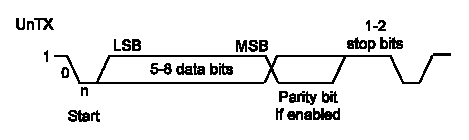
\includegraphics[width=0.5\textwidth] {figuras/uartTiva.eps}
	\caption{Sinal de Transmissão UART no Tiva TM4C1294NCPDT}
	\label{fig:uartTiva}
\end{figure}

A figura \ref{tab:CanaisUART} apresenta os pinos de entrada e saída do UART que podem ser usados no Tiva TM4C1294NCPDT.
  
\begin{table}[H]
	\centering
	\caption{Canais do UART - Tiva TM4C1294NCPDT \cite{DATASHEET_TIVA} }
	\label{tab:CanaisUART}
	\begin{tabular}{|c|c|c|c|l|}
		\rowcolor[HTML]{000000} 
		{\color[HTML]{FFFFFF} Pino}  & {\color[HTML]{FFFFFF} Mux/Função} & {\color[HTML]{FFFFFF} Tipo} & {\color[HTML]{FFFFFF} Buffer} & {\color[HTML]{FFFFFF} Descrição}  \\
		\hline
		UORx  & PA0 (1) & I & TTL & UART Módulo 0, recepção do sinal   \\
		\hline
		U0Tx  & PA1 (1) & O & TTL & UART Módulo 0, transmissão do sinal  \\
		\hline
		\hline
		U1Rx  & PB0 (1) & I & TTL & UART Módulo 1, recepção do sinal   \\
		      & PQ4 (1) &   &     &                                     \\
		\hline
		U1Tx  & PB1 (1) & O & TTL & UART Módulo 1, transmissão do sinal  \\
		\hline
		U2Rx  & PA6 (1) & I & TTL & UART Módulo 2, recepção do sinal   \\
		      & PD4 (1) &   &     &                                      \\
		\hline
		U2Tx  & PA7 (1) & O & TTL & UART Módulo 2, transmissão do sinal  \\
		      & PD5 (1) &   &     &                                      \\
		\hline
		U3Rx  & PA4 (1) (1) & I & TTL & UART Módulo 3, recepção do sinal   \\
	 	      & PJ0 (1) &   &     &                                      \\
		\hline
		U3Tx  & PA5 (1) & O & TTL & UART Módulo 3, transmissão do sinal  \\
	 	      & PJ1 (1) &   &     &                                      \\
		\hline
		U4Rx  & PK0 (1) & I & TTL & UART Módulo 4, recepção do sinal   \\
		      & PA2 (1) &   &     &                                      \\
		\hline
		U4Tx  & PK1 (1) & O & TTL & UART Módulo 4, transmissão do sinal  \\
		      & PA3 (1) &   &     &                                      \\
		\hline
		U5Rx  & PC6 (1) & I & TTL & UART Módulo 5, recepção do sinal\\
		\hline
		U5Tx  & PC7 (1) & O & TTL & UART Módulo 5, transmissão do sinal \\
		\hline
		U6Rx  & PP0 (1) & I & TTL & UART Módulo 6, recepção do sinal \\
		\hline
		U6Tx  & PP1 (1) & O & TTL & UART Módulo 6, transmissão do sinal\\
		\hline
		U7Rx  & PC4 (1) & I & TTL & UART Módulo 7, recepção do sinal \\
		\hline
		U7Tx  & PC5 (1) & O & TTL & UART Módulo 7, transmissão do sinal\\
		\hline
	\end{tabular}
\end{table}


\section{Na TivaWare}

